\documentclass[aspectratio=169,11pt]{beamer}

\usetheme{Madrid}
\usecolortheme{default}
\setbeamercovered{transparent}

\usepackage{graphicx}
\usepackage{amsmath}
\usepackage{amssymb}
\usepackage{booktabs}
\usepackage{tikz}
\usetikzlibrary{arrows.meta, shapes.geometric, positioning,
                fit, backgrounds, shadows.blur,
                decorations.pathreplacing, calc}

\setbeamersize{text margin left=0.6cm, text margin right=0.6cm}
\setlength{\leftmargini}{0.9em}
\setlength{\leftmarginii}{1.4em}

\tikzset{
  pipenode/.style={
    rectangle, rounded corners=4pt,
    minimum width=1.6cm, minimum height=0.9cm,
    text centered, font=\scriptsize\bfseries,
    draw=#1!70!black, fill=#1!30, text=#1!20!black,
    drop shadow
  },
  pipearrow/.style={-Stealth, thick, color=gray!70},
  sysbox/.style={
    rectangle, rounded corners=5pt,
    minimum width=2.8cm, minimum height=0.85cm,
    text centered, font=\scriptsize\bfseries,
    draw=#1!70!black, fill=#1!25, text=#1!20!black,
    drop shadow
  },
  flowbox/.style={
    rectangle, rounded corners=4pt,
    minimum width=3.2cm, minimum height=0.7cm,
    text centered, font=\scriptsize,
    draw=blue!50!black, fill=blue!10, text=blue!20!black
  },
  sdgbox/.style={
    rectangle, rounded corners=6pt,
    minimum width=3.5cm, minimum height=1.0cm,
    text centered, font=\scriptsize\bfseries,
    draw=#1!70!black, fill=#1!20, text=#1!20!black,
    drop shadow
  },
  metricbox/.style={
    rectangle, rounded corners=5pt,
    minimum width=2.6cm, minimum height=1.4cm,
    text centered, font=\small\bfseries,
    draw=#1!70!black, fill=#1!20, text=#1!20!black,
    drop shadow
  },
}

\title{Brain Tumour Detection Using\\Convolutional Neural Networks}
\subtitle{CEP: Artificial Intelligence and Machine Learning Lab}
\author{%
  Muhammad Ahmad~{\small(FA23-BCE-113)}\\[2pt]
  Uzair~{\small(FA23-BCE-098)}%
}
\date{\today}
\institute{Computer Engineering Department\\COMSATS University Islamabad -- Lahore Campus}

\begin{document}

\begin{document}
% ── Custom footer ─────────────────────────────────────────────────────────────
\setbeamertemplate{footline}{%
  \leavevmode%
  \hbox{%
    % Left empty block
    \begin{beamercolorbox}[wd=0.20\paperwidth, ht=2.5ex, dp=1.5ex,
                           leftskip=0.3cm]{author in head/foot}%
    \end{beamercolorbox}%
    % Centre block: project name
    \begin{beamercolorbox}[wd=0.60\paperwidth, ht=2.5ex, dp=1.5ex,
                           center]{title in head/foot}%
      \usebeamerfont{title in head/foot}%
      \textbf{Cancer Cell Detection Pipeline}%
    \end{beamercolorbox}%
    % Right block: slide number
    \begin{beamercolorbox}[wd=0.20\paperwidth, ht=2.5ex, dp=1.5ex,
                           rightskip=0.3cm, right]{date in head/foot}%
      \usebeamerfont{date in head/foot}%
      \insertframenumber{} / \inserttotalframenumber%
    \end{beamercolorbox}%
  }%
  \vskip0pt%
}
% ===== TITLE =====
\begin{frame}
    \titlepage
\end{frame}

% ===== OUTLINE =====
\begin{frame}{Outline}
    \tableofcontents
\end{frame}

% ===== SECTION 1 =====
\section{Introduction}

\begin{frame}{Problem Statement}
    \begin{itemize}\setlength\itemsep{4pt}
        \item \textbf{Challenge:} Early cancer detection is crucial for patient survival
        
        \item Medical image analysis is time-consuming and requires expert radiologists
        
        \item Manual analysis is prone to human error and variability
        
        \item Limited access to specialised expertise in resource-constrained regions
        
        \item \textbf{Solution:} Automated image processing pipeline for objective feature extraction
    \end{itemize}
    \vspace{0.3cm}
    \begin{center}
        \small\textit{Objective: Develop a robust, multi-stage image processing system
        for automated medical image analysis}
    \end{center}
\end{frame}

\begin{frame}{Key Objectives}
    \begin{columns}[T]
        \column{0.48\textwidth}
        \textbf{Primary Goals:}
        \begin{itemize}\setlength\itemsep{3pt}
            \item Enhance diagnostic image contrast
            \item Extract structural features
            \item Identify tumour boundaries
            \item Reduce noise and artefacts
            \item Enable multi-aspect analysis
        \end{itemize}
        \column{0.48\textwidth}
        \textbf{Technical Requirements:}
        \begin{itemize}\setlength\itemsep{3pt}
            \item Scalable microservices architecture
            \item Real-time processing capability
            \item Cloud infrastructure integration
            \item Quantitative quality metrics
            \item Clinical validation support
        \end{itemize}
    \end{columns}
    \vspace{0.4cm}
    \centering
    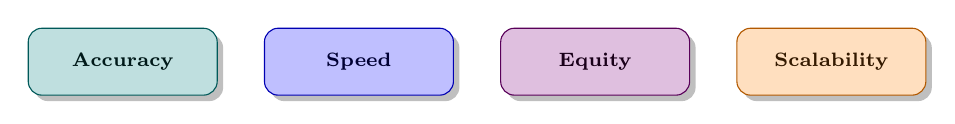
\begin{tikzpicture}
      \node[sysbox=teal,   minimum width=2.4cm] at (0,0)   {Accuracy};
      \node[sysbox=blue,   minimum width=2.4cm] at (3.0,0) {Speed};
      \node[sysbox=violet, minimum width=2.4cm] at (6.0,0) {Equity};
      \node[sysbox=orange, minimum width=2.4cm] at (9.0,0) {Scalability};
    \end{tikzpicture}
\end{frame}
% ===== SECTION 2 =====
\section{System Architecture}

\begin{frame}{System Architecture Overview}

\centering

\scalebox{0.35}{
    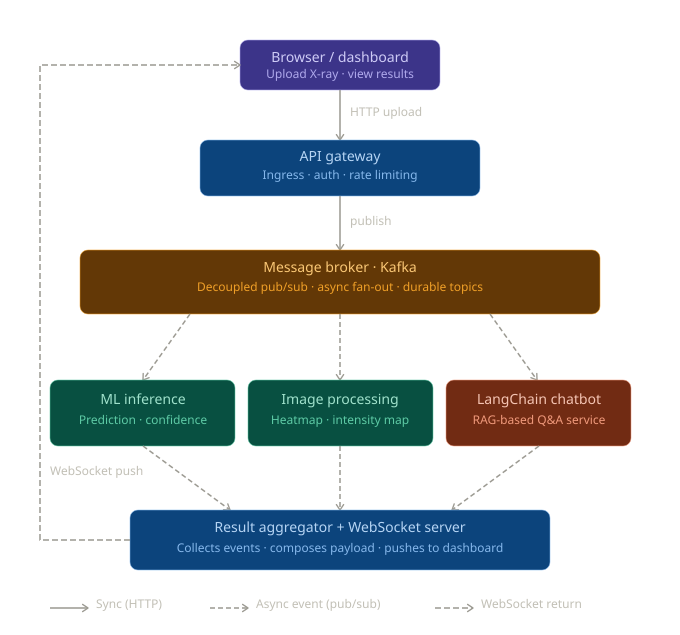
\includegraphics{image-processor/event_driven_xray_architecture.png}
}
\end{frame}


\begin{frame}{Data Processing Flow}
  \centering
  \vspace{0.15cm}
  \begin{tikzpicture}[
      every node/.style={font=\scriptsize},
      step/.style={
        rectangle, rounded corners=3pt,
        minimum width=8.5cm, minimum height=0.52cm,
        text centered
      }
    ]

    \node[step, fill=gray!15,   draw=gray!55]
         (s1) at (0, 0.00) {1.\ Upload Medical Image};

    \node[step, fill=blue!12,   draw=blue!55]
         (s2) at (0,-0.80) {2.\ API Gateway Validates and Routes Request};

    \node[step, fill=teal!12,   draw=teal!55]
         (s3) at (0,-1.60) {3.\ Image Processor applies 6-Stage Transformation};

    \node[step, fill=red!12,    draw=red!55]
         (s4) at (0,-2.40) {4.\ Results Published to Apache Kafka Queue};

    \node[step, fill=violet!12, draw=violet!55]
         (s5) at (0,-3.20) {5.\ ML Service Consumes Features for Classification};

    \node[step, fill=green!12,  draw=green!55]
         (s6) at (0,-4.00) {6.\ Result Aggregator Persists to PostgreSQL};

    \node[step, fill=orange!12, draw=orange!55]
         (s7) at (0,-4.80) {7.\ Results Returned to User Dashboard};

    \draw[pipearrow] (s1.south)--(s2.north);
    \draw[pipearrow] (s2.south)--(s3.north);
    \draw[pipearrow] (s3.south)--(s4.north);
    \draw[pipearrow] (s4.south)--(s5.north);
    \draw[pipearrow] (s5.south)--(s6.north);
    \draw[pipearrow] (s6.south)--(s7.north);

  \end{tikzpicture}
\end{frame}
\begin{frame}{6-Stage Image Processing Pipeline}
  \centering
  \vspace{0.2cm}

  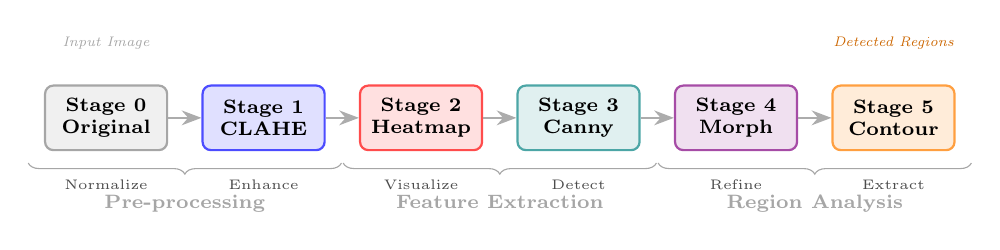
\begin{tikzpicture}[
      stage/.style={
        rectangle, rounded corners=3pt,
        minimum width=1.55cm, minimum height=0.82cm,
        align=center, font=\scriptsize\bfseries,
        line width=0.8pt
      },
      note/.style={
        font=\tiny, text=black!70, align=center
      },
      arr/.style={
        -{Stealth[length=2.5mm]}, line width=0.9pt, draw=gray!65
      }
    ]

    % --- Stage boxes ---
    \node[stage, draw=gray!70,   fill=gray!12]   (s0) at (0.0,0)   {Stage 0\\Original};
    \node[stage, draw=blue!70,   fill=blue!12]   (s1) at (2.0,0)   {Stage 1\\CLAHE};
    \node[stage, draw=red!70,    fill=red!12]    (s2) at (4.0,0)   {Stage 2\\Heatmap};
    \node[stage, draw=teal!70,   fill=teal!12]   (s3) at (6.0,0)   {Stage 3\\Canny};
    \node[stage, draw=violet!70, fill=violet!12] (s4) at (8.0,0)   {Stage 4\\Morph};
    \node[stage, draw=orange!75, fill=orange!15] (s5) at (10.0,0)  {Stage 5\\Contour};

    % --- Arrows ---
    \draw[arr] (s0.east) -- (s1.west);
    \draw[arr] (s1.east) -- (s2.west);
    \draw[arr] (s2.east) -- (s3.west);
    \draw[arr] (s3.east) -- (s4.west);
    \draw[arr] (s4.east) -- (s5.west);

    % --- Short notes under each stage ---
    \node[note] at (0.0,-0.85)  {Normalize};
    \node[note] at (2.0,-0.85)  {Enhance};
    \node[note] at (4.0,-0.85)  {Visualize};
    \node[note] at (6.0,-0.85)  {Detect};
    \node[note] at (8.0,-0.85)  {Refine};
    \node[note] at (10.0,-0.85) {Extract};

    % --- Input / Output labels ---
    \node[font=\tiny\itshape, text=gray!70]   at (0.0,0.95)  {Input Image};
    \node[font=\tiny\itshape, text=orange!80!black] at (10.0,0.95) {Detected Regions};

    % --- Phase grouping braces ---
    \draw[decorate, decoration={brace, mirror, amplitude=4pt}, gray!70]
      ([xshift=-0.20cm,yshift=-0.15cm]s0.south west) --
      ([xshift= 0.20cm,yshift=-0.15cm]s1.south east)
      node[midway, below=8pt, font=\scriptsize\bfseries] {Pre-processing};

    \draw[decorate, decoration={brace, mirror, amplitude=4pt}, gray!70]
      ([xshift=-0.20cm,yshift=-0.15cm]s2.south west) --
      ([xshift= 0.20cm,yshift=-0.15cm]s3.south east)
      node[midway, below=8pt, font=\scriptsize\bfseries] {Feature Extraction};

    \draw[decorate, decoration={brace, mirror, amplitude=4pt}, gray!70]
      ([xshift=-0.20cm,yshift=-0.15cm]s4.south west) --
      ([xshift= 0.20cm,yshift=-0.15cm]s5.south east)
      node[midway, below=8pt, font=\scriptsize\bfseries] {Region Analysis};

  \end{tikzpicture}
\end{frame}

% ===== STAGE 0 =====
\begin{frame}{Stage 0: Original Image}
    \begin{columns}[T]
        \column{0.52\textwidth}
        \textbf{Grayscale Normalisation:}
        \begin{itemize}\setlength\itemsep{4pt}
            \item Load image as 8-bit grayscale (0--255)
            \item Normalise: $I_{norm} = \dfrac{I_{original}}{255}$
            \item Establish baseline for subsequent stages
            \item Compute intensity histogram
        \end{itemize}
        \vspace{0.3cm}
        \textbf{Key Information:}
        \begin{itemize}\setlength\itemsep{3pt}
            \item Reference for PSNR and MSE
            \item Baseline for all comparisons
            \item Histogram shows distribution
        \end{itemize}
        \column{0.44\textwidth}
        \centering\vspace{0.3cm}
    \end{columns}
\end{frame}

\begin{frame}{Stage 0: Original Grayscale Image and Histogram}
    \centering
    
\includegraphics[width=0.96\textwidth,height=0.80\textheight,
                     keepaspectratio]{image-processor/original_with_histogram.png}
\end{frame}

% ===== STAGE 1 =====
\begin{frame}{Stage 1: CLAHE Enhancement}
    \begin{columns}[T]
        \column{0.52\textwidth}
        \textbf{Algorithm:}
        \begin{itemize}\setlength\itemsep{4pt}
            \item Divide image into 8$\times$8 tiles
            \item Per-tile histogram equalisation
            \item Clipping limit = 2.0
            \item Interpolate between tile boundaries
        \end{itemize}
        \vspace{0.3cm}
        \textbf{Benefits:}
        \begin{itemize}\setlength\itemsep{3pt}
            \item Enhanced local contrast
            \item Prevents noise amplification
            \item Reveals subtle features
            \item Maintains natural appearance
        \end{itemize}
        \column{0.44\textwidth}
        \centering\vspace{0.3cm}
        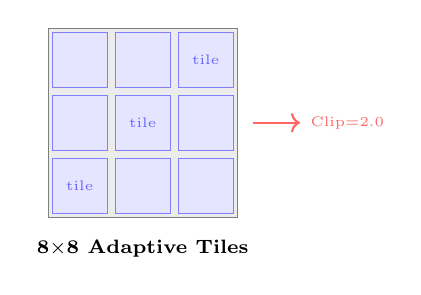
\begin{tikzpicture}
          \draw[fill=gray!15,draw=gray](0,0)rectangle(2.4,2.4);
          \draw[blue!50,fill=blue!10](0.05,0.05)rectangle(0.75,0.75);
          \draw[blue!50,fill=blue!10](0.85,0.05)rectangle(1.55,0.75);
          \draw[blue!50,fill=blue!10](1.65,0.05)rectangle(2.35,0.75);
          \draw[blue!50,fill=blue!10](0.05,0.85)rectangle(0.75,1.55);
          \draw[blue!50,fill=blue!10](0.85,0.85)rectangle(1.55,1.55);
          \draw[blue!50,fill=blue!10](1.65,0.85)rectangle(2.35,1.55);
          \draw[blue!50,fill=blue!10](0.05,1.65)rectangle(0.75,2.35);
          \draw[blue!50,fill=blue!10](0.85,1.65)rectangle(1.55,2.35);
          \draw[blue!50,fill=blue!10](1.65,1.65)rectangle(2.35,2.35);
          \node[font=\tiny,text=blue!60]at(0.4,0.4){tile};
          \node[font=\tiny,text=blue!60]at(1.2,1.2){tile};
          \node[font=\tiny,text=blue!60]at(2.0,2.0){tile};
          \node[font=\scriptsize\bfseries,below=2pt]at(1.2,-0.1){8$\times$8 Adaptive Tiles};
          \draw[red!60,thick,->](2.6,1.2)--(3.2,1.2)
               node[right,font=\tiny,text=red!60]{Clip=2.0};
        \end{tikzpicture}
    \end{columns}
\end{frame}

\begin{frame}{Stage 1: CLAHE Enhancement Result}
    \centering
    
\includegraphics[width=0.96\textwidth,height=0.80\textheight,
                     keepaspectratio]{image-processor/clahe_with_histogram.png}
\end{frame}

% ===== STAGE 2 =====
\begin{frame}{Stage 2: Heatmap Visualisation}
    \begin{columns}[T]
        \column{0.52\textwidth}
        \textbf{JET Colour Mapping:}
        \begin{itemize}\setlength\itemsep{4pt}
            \item Apply JET colourmap (blue to red)
            \item Dark colours: low intensity (background)
            \item Bright colours: high intensity (tumours)
        \end{itemize}
        \vspace{0.3cm}
        \textbf{Clinical Application:}
        \begin{itemize}\setlength\itemsep{3pt}
            \item Rapid hotspot identification
            \item Intuitive visual representation
            \item Radiologist interpretation aid
        \end{itemize}
        \column{0.44\textwidth}
        \centering\vspace{0.2cm}
        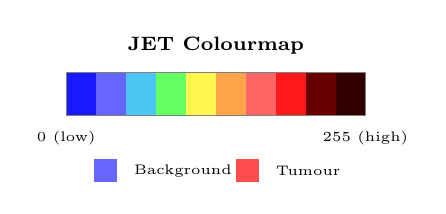
\begin{tikzpicture}
          \fill[blue!90]      (0.00,0)rectangle(0.38,0.55);
          \fill[blue!60]      (0.38,0)rectangle(0.76,0.55);
          \fill[cyan!70]      (0.76,0)rectangle(1.14,0.55);
          \fill[green!60]     (1.14,0)rectangle(1.52,0.55);
          \fill[yellow!70]    (1.52,0)rectangle(1.90,0.55);
          \fill[orange!70]    (1.90,0)rectangle(2.28,0.55);
          \fill[red!60]       (2.28,0)rectangle(2.66,0.55);
          \fill[red!90]       (2.66,0)rectangle(3.04,0.55);
          \fill[red!40!black] (3.04,0)rectangle(3.42,0.55);
          \fill[red!20!black] (3.42,0)rectangle(3.80,0.55);
          \draw[gray](0,0)rectangle(3.8,0.55);
          \node[font=\tiny,below=2pt]at(0,0){0 (low)};
          \node[font=\tiny,below=2pt]at(3.8,0){255 (high)};
          \node[font=\scriptsize\bfseries,above=3pt]at(1.9,0.55){JET Colourmap};
          \node[rectangle,fill=blue!60,minimum width=0.3cm,
                minimum height=0.3cm](lb)at(0.5,-0.7){};
          \node[right=0.08cm of lb,font=\tiny]{Background};
          \node[rectangle,fill=red!70,minimum width=0.3cm,
                minimum height=0.3cm](lr)at(2.3,-0.7){};
          \node[right=0.08cm of lr,font=\tiny]{Tumour};
        \end{tikzpicture}
    \end{columns}
\end{frame}

\begin{frame}{Stage 2: Heatmap Visualisation Result}
    \centering
    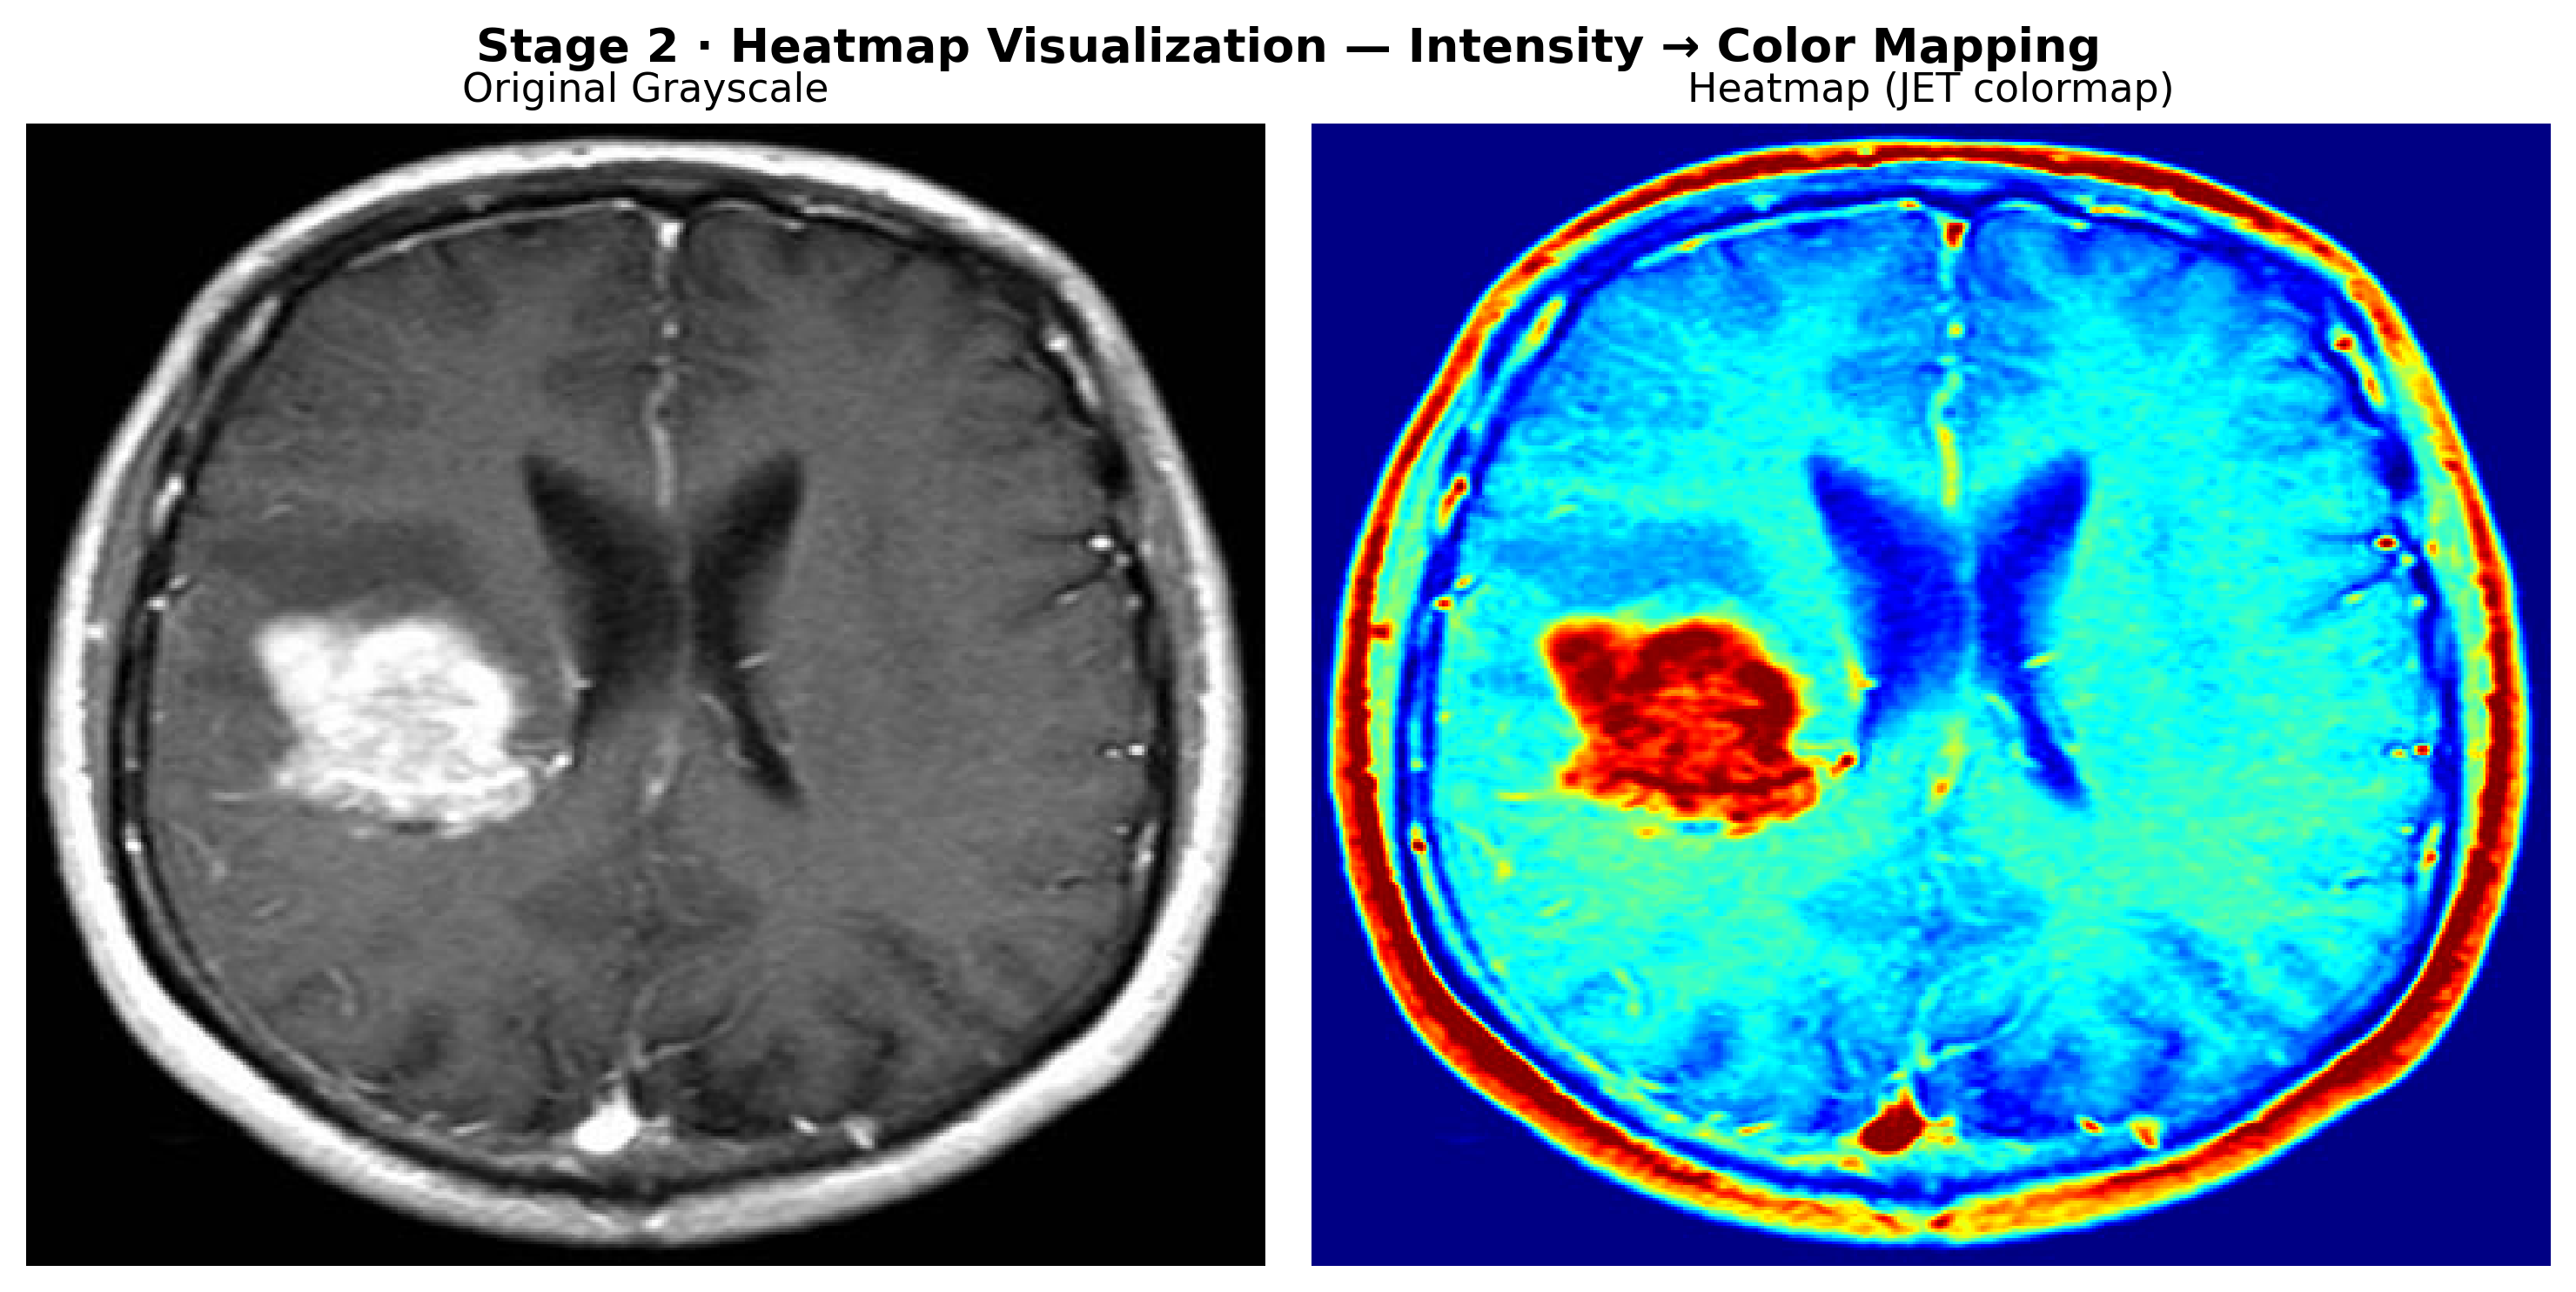
\includegraphics[width=0.96\textwidth,height=0.80\textheight,
                     keepaspectratio]{image-processor/heatmap_comparison.png}
\end{frame}

% ===== STAGE 3 =====
\begin{frame}{Stage 3: Canny Edge Detection}
    \begin{columns}[T]
        \column{0.52\textwidth}
        \textbf{Algorithm Steps:}
        \begin{itemize}\setlength\itemsep{3pt}
            \item Gaussian blur for noise reduction
            \item Sobel gradient in x and y directions
            \item Non-maximum suppression
            \item Hysteresis thresholding (100, 200)
        \end{itemize}
        \vspace{0.2cm}
        \textbf{Advantages:}
        \begin{itemize}\setlength\itemsep{3pt}
            \item Precise structural boundaries
            \item Low false-positive rate
            \item Connected edge chains
            \item Robust to noise
        \end{itemize}
        \column{0.44\textwidth}
        \centering\vspace{0.1cm}
        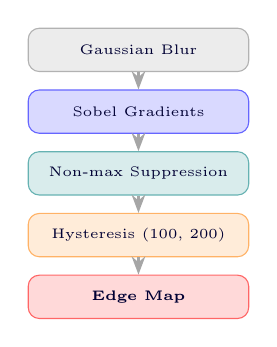
\begin{tikzpicture}[node distance=0.28cm]
          \node[flowbox,fill=gray!15,draw=gray!60,minimum width=2.8cm,
                minimum height=0.55cm,font=\tiny](g){Gaussian Blur};
          \node[flowbox,fill=blue!15,draw=blue!60,minimum width=2.8cm,
                minimum height=0.55cm,font=\tiny,below=0.22cm of g](s){Sobel Gradients};
          \node[flowbox,fill=teal!15,draw=teal!60,minimum width=2.8cm,
                minimum height=0.55cm,font=\tiny,below=0.22cm of s](n){Non-max Suppression};
          \node[flowbox,fill=orange!15,draw=orange!60,minimum width=2.8cm,
                minimum height=0.55cm,font=\tiny,below=0.22cm of n](h){Hysteresis (100, 200)};
          \node[flowbox,fill=red!15,draw=red!60,minimum width=2.8cm,
                minimum height=0.55cm,font=\tiny\bfseries,below=0.22cm of h](e){Edge Map};
          \draw[pipearrow](g.south)--(s.north);
          \draw[pipearrow](s.south)--(n.north);
          \draw[pipearrow](n.south)--(h.north);
          \draw[pipearrow](h.south)--(e.north);
        \end{tikzpicture}
    \end{columns}
\end{frame}

\begin{frame}{Stage 3: Canny Edge Detection Result}
    \centering
    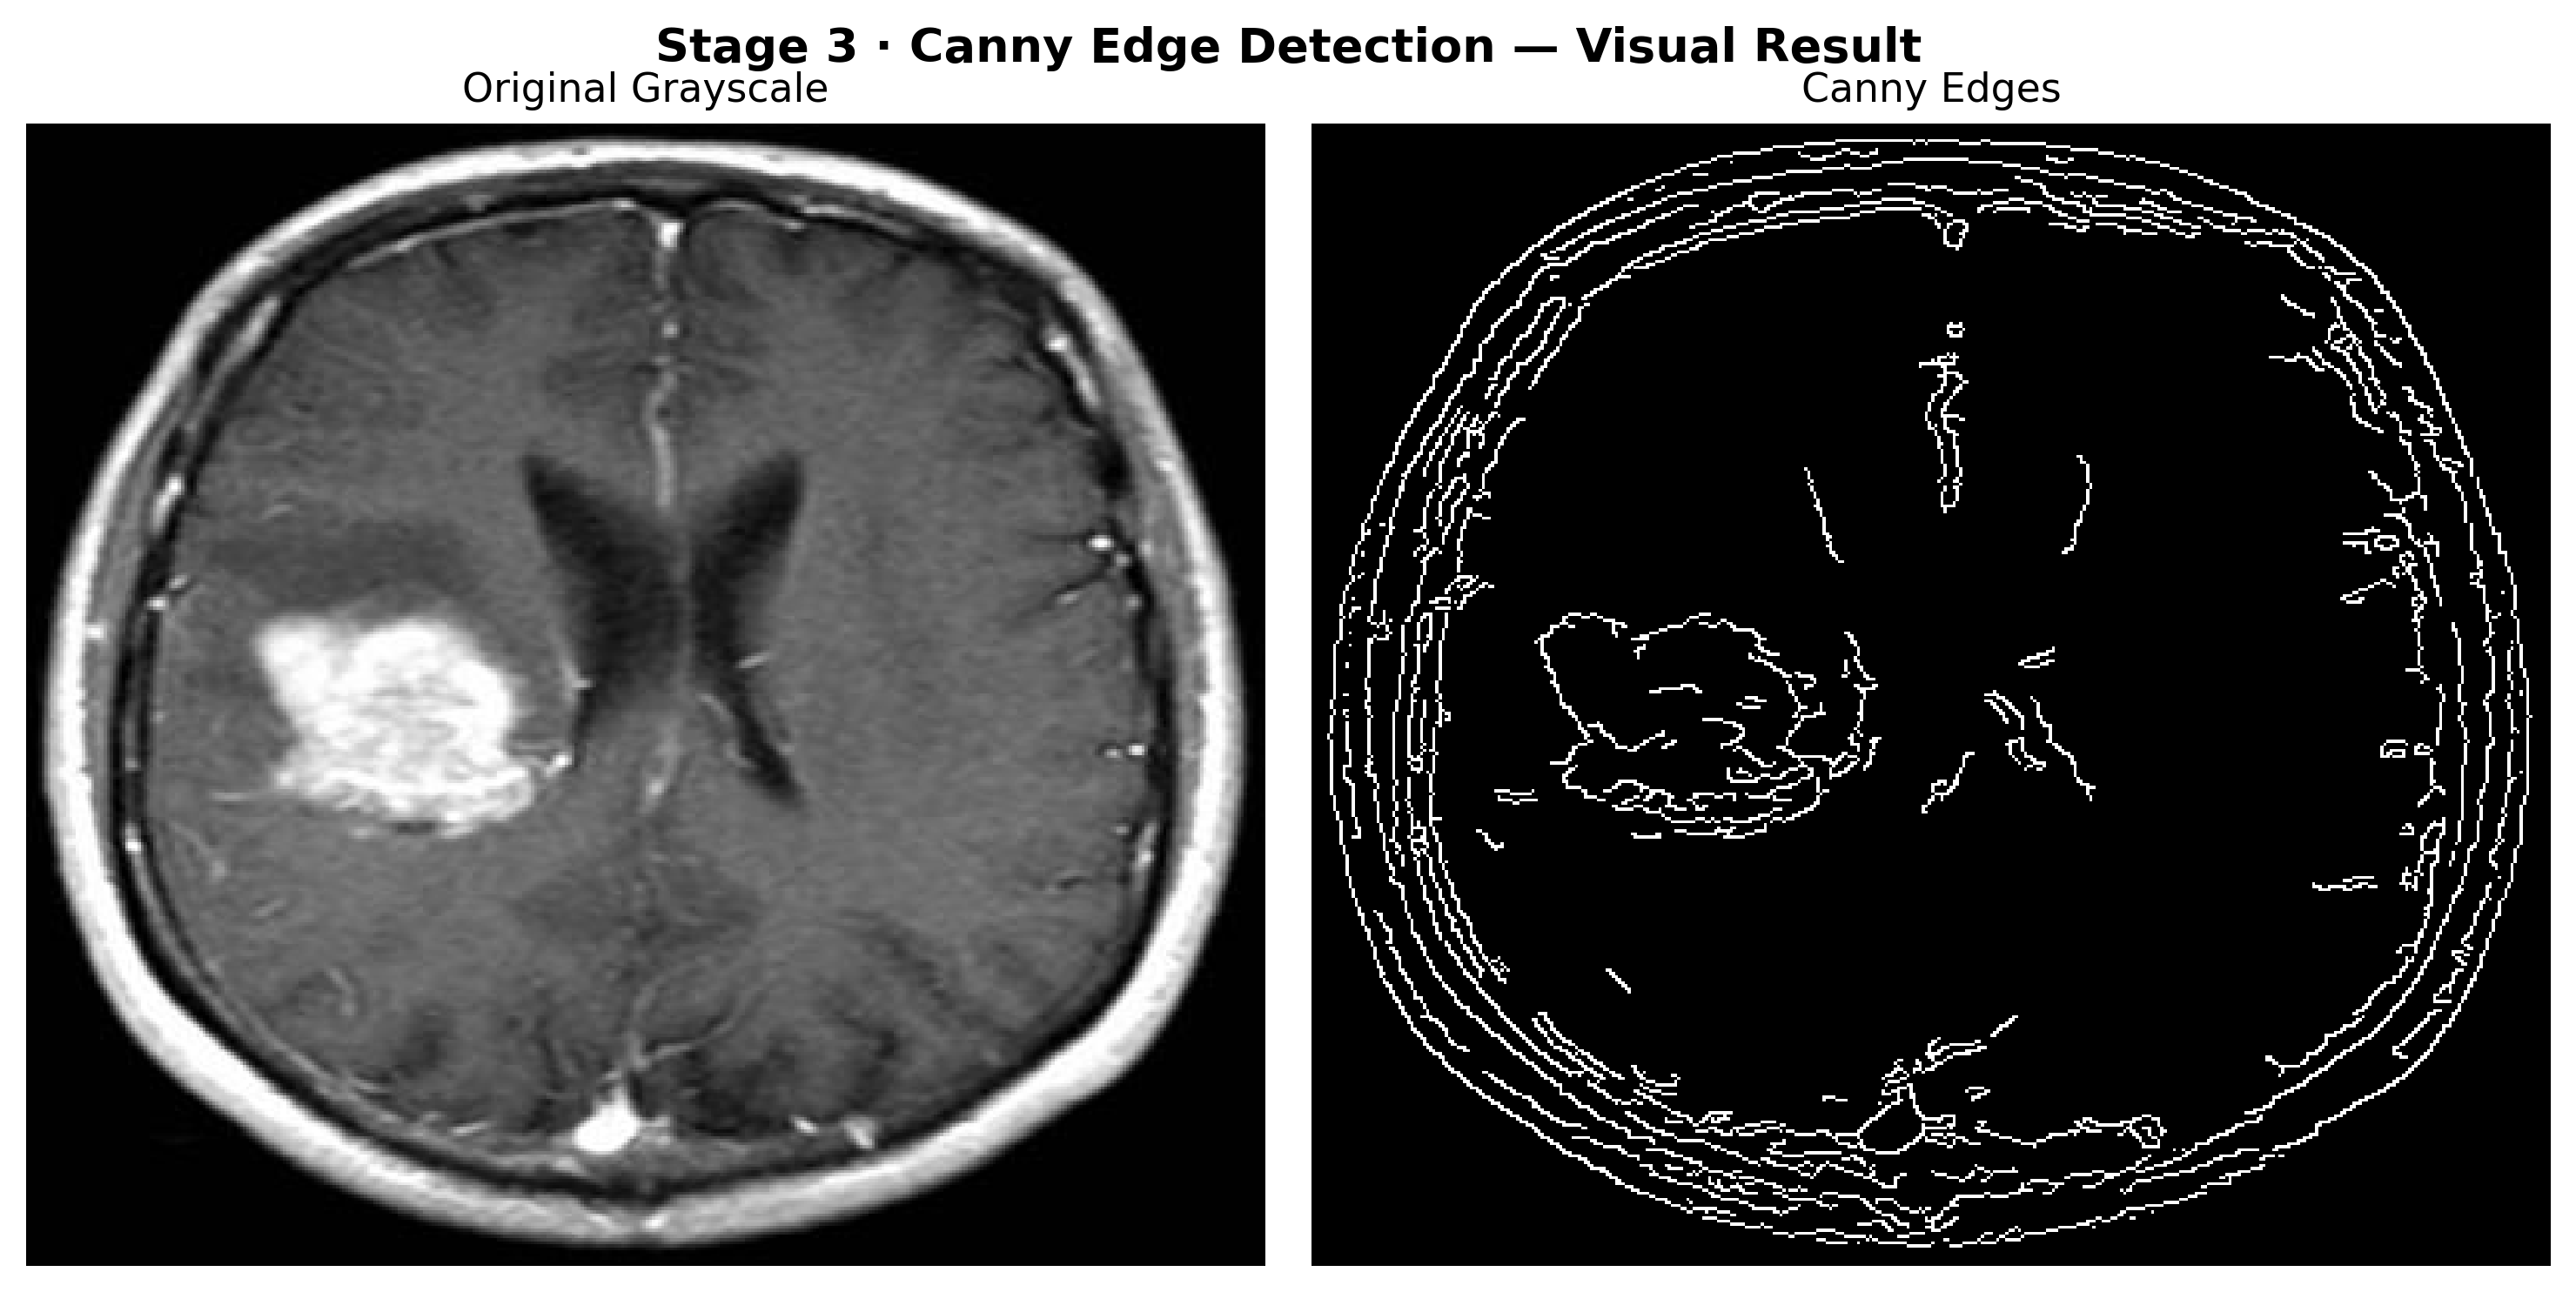
\includegraphics[width=0.96\textwidth,height=0.80\textheight,
                     keepaspectratio]{image-processor/canny_comparison.png}
\end{frame}

% ===== STAGE 4 =====
\begin{frame}{Stage 4: Morphological Operations}
    \begin{columns}[T]
        \column{0.52\textwidth}
        \textbf{Filtering Sequence:}
        \begin{enumerate}\setlength\itemsep{3pt}
            \item Binary threshold (= 127)
            \item Opening: Erosion then Dilation
            \item Closing: Dilation then Erosion
            \item Kernel: 5$\times$5 elliptical element
        \end{enumerate}
        \vspace{0.2cm}
        \textbf{Effects:}
        \begin{itemize}\setlength\itemsep{3pt}
            \item Removes small artefacts
            \item Fills holes in regions
            \item Preserves main structures
        \end{itemize}
        \column{0.44\textwidth}
        \centering\vspace{0.2cm}
        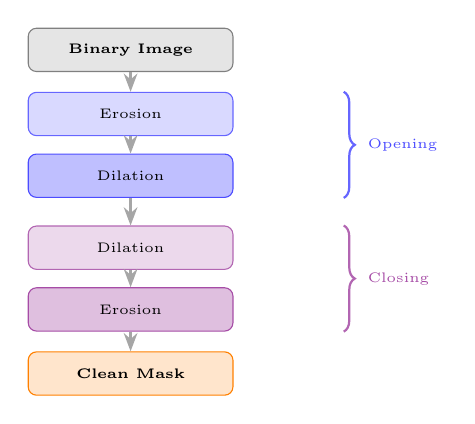
\begin{tikzpicture}[node distance=0.3cm]
          \node[rectangle,rounded corners=3pt,fill=gray!20,draw=gray,
                minimum width=2.6cm,minimum height=0.55cm,
                font=\tiny\bfseries](bin){Binary Image};
          \node[rectangle,rounded corners=3pt,fill=blue!15,draw=blue!60,
                minimum width=2.6cm,minimum height=0.55cm,
                font=\tiny,below=0.25cm of bin](er1){Erosion};
          \node[rectangle,rounded corners=3pt,fill=blue!25,draw=blue!70,
                minimum width=2.6cm,minimum height=0.55cm,
                font=\tiny,below=0.22cm of er1](di1){Dilation};
          \draw[decorate,decoration={brace,amplitude=4pt},blue!60,thick]
               ([xshift=1.4cm]er1.north east)--([xshift=1.4cm]di1.south east)
               node[midway,right=5pt,font=\tiny,text=blue!70]{Opening};
          \node[rectangle,rounded corners=3pt,fill=violet!15,draw=violet!60,
                minimum width=2.6cm,minimum height=0.55cm,
                font=\tiny,below=0.35cm of di1](di2){Dilation};
          \node[rectangle,rounded corners=3pt,fill=violet!25,draw=violet!70,
                minimum width=2.6cm,minimum height=0.55cm,
                font=\tiny,below=0.22cm of di2](er2){Erosion};
          \draw[decorate,decoration={brace,amplitude=4pt},violet!60,thick]
               ([xshift=1.4cm]di2.north east)--([xshift=1.4cm]er2.south east)
               node[midway,right=5pt,font=\tiny,text=violet!70]{Closing};
          \node[rectangle,rounded corners=3pt,fill=orange!20,draw=orange,
                minimum width=2.6cm,minimum height=0.55cm,
                font=\tiny\bfseries,below=0.25cm of er2](out){Clean Mask};
          \draw[pipearrow](bin.south)--(er1.north);
          \draw[pipearrow](er1.south)--(di1.north);
          \draw[pipearrow](di1.south)--(di2.north);
          \draw[pipearrow](di2.south)--(er2.north);
          \draw[pipearrow](er2.south)--(out.north);
        \end{tikzpicture}
    \end{columns}
\end{frame}

\begin{frame}{Stage 4: Morphological Operations Result}
    \centering
    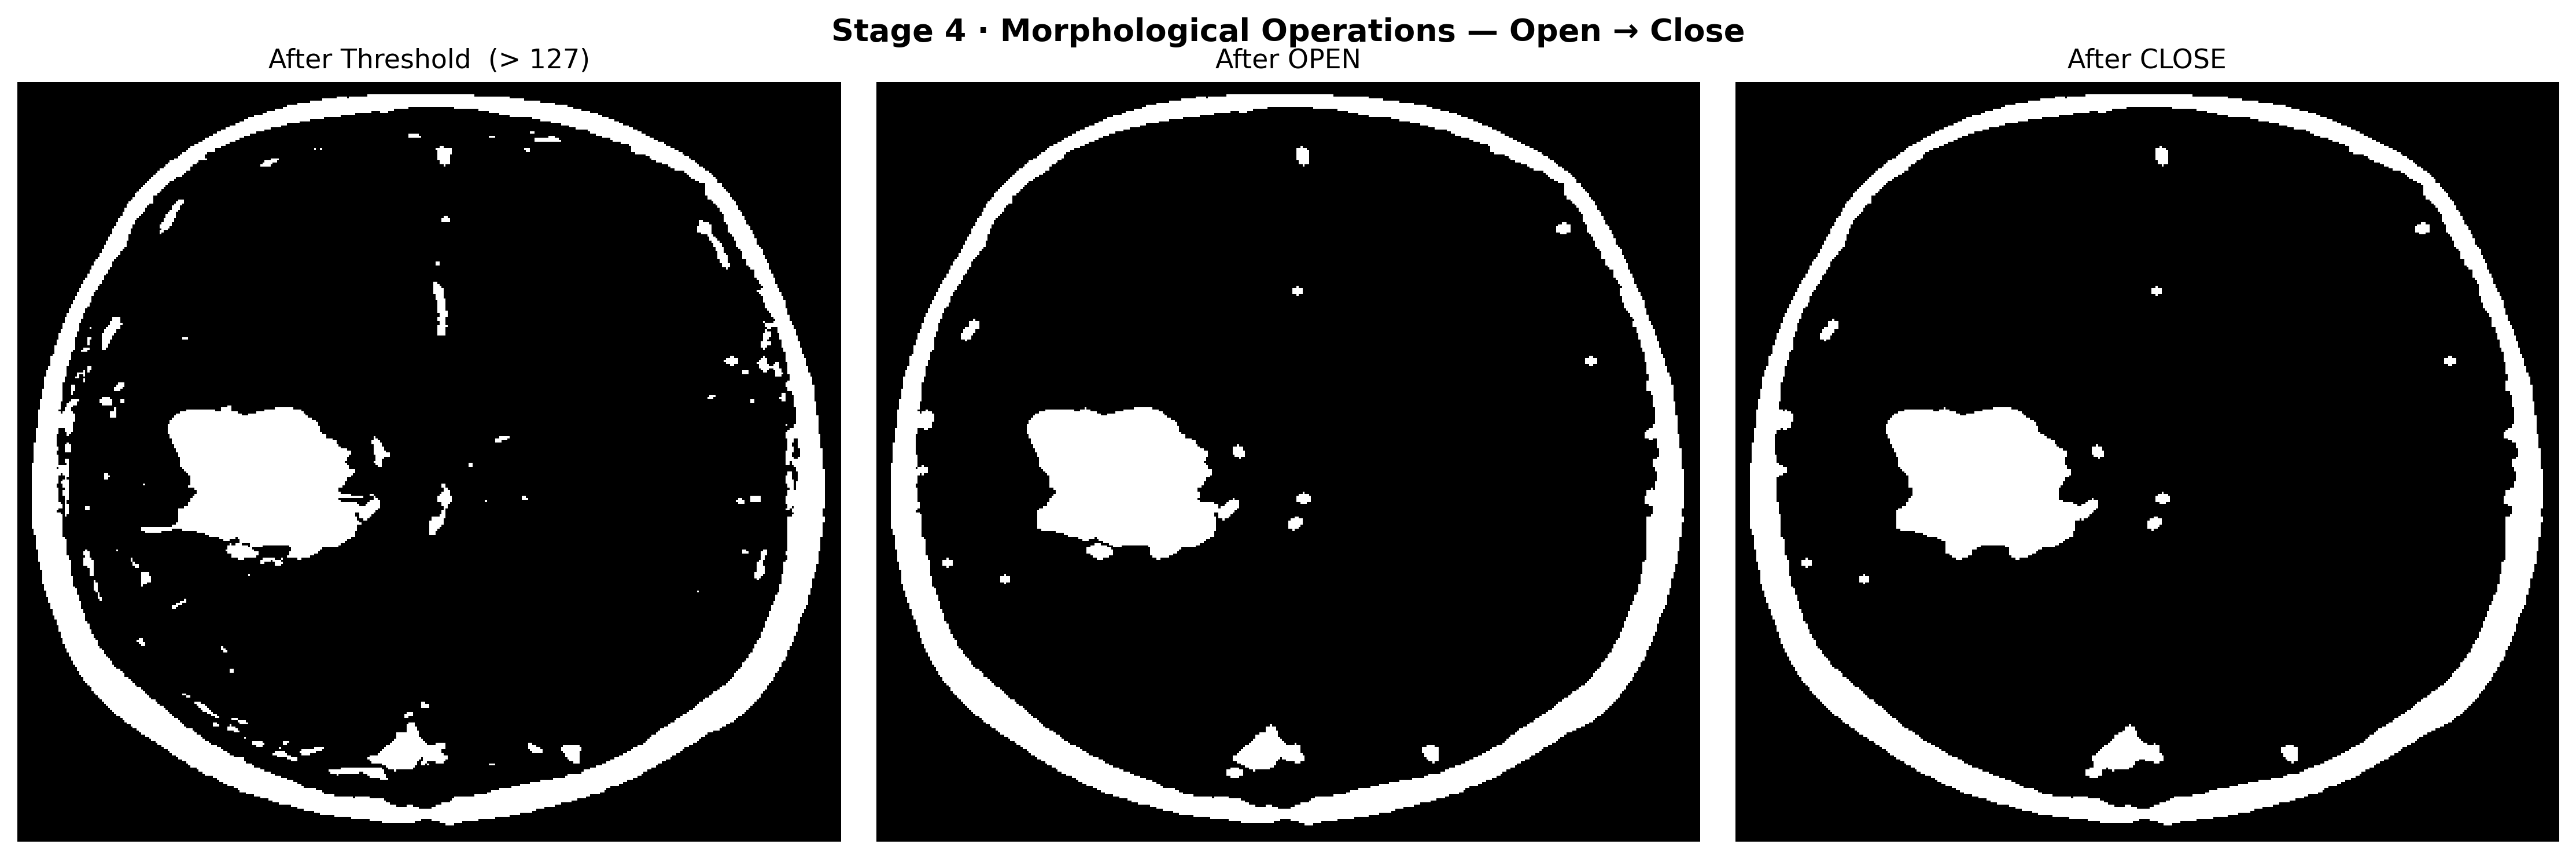
\includegraphics[width=0.96\textwidth,height=0.80\textheight,
                     keepaspectratio]{image-processor/morphological_steps.png}
\end{frame}

% ===== STAGE 5 =====
\begin{frame}{Stage 5: Contour Detection}
    \begin{columns}[T]
        \column{0.52\textwidth}
        \textbf{Connected Component Analysis:}
        \begin{itemize}\setlength\itemsep{4pt}
            \item Find contours in binary image
            \item Filter by area (minimum 100 pixels)
            \item Extract boundary coordinates
            \item Compute shape properties
        \end{itemize}
        \vspace{0.2cm}
        \textbf{Output Features:}
        \begin{itemize}\setlength\itemsep{3pt}
            \item Tumour regions identified
            \item Boundary coordinates extracted
            \item Area and perimeter computed
            \item Feature vectors for ML
        \end{itemize}
        \column{0.44\textwidth}
        \centering\vspace{0.2cm}
        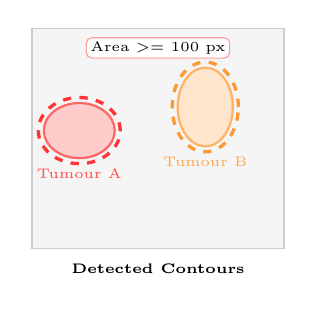
\begin{tikzpicture}
          \draw[fill=gray!8,draw=gray!40](0,0)rectangle(3.2,2.8);
          \draw[fill=red!20,draw=red!60,thick](0.6,1.5)ellipse(0.45 and 0.35);
          \draw[red!80,dashed,very thick](0.6,1.5)ellipse(0.52 and 0.42);
          \node[font=\tiny,text=red!70]at(0.6,0.95){Tumour A};
          \draw[fill=orange!20,draw=orange!60,thick](2.2,1.8)ellipse(0.35 and 0.5);
          \draw[orange!80,dashed,very thick](2.2,1.8)ellipse(0.42 and 0.57);
          \node[font=\tiny,text=orange!70]at(2.2,1.1){Tumour B};
          \node[font=\tiny,fill=white,draw=red!40,rounded corners=2pt,
                inner sep=1.5pt]at(1.6,2.55){Area >= 100 px};
          \node[font=\tiny\bfseries]at(1.6,-0.25){Detected Contours};
        \end{tikzpicture}
    \end{columns}
\end{frame}

\begin{frame}{Stage 5: Contour Detection Result}
    \centering
    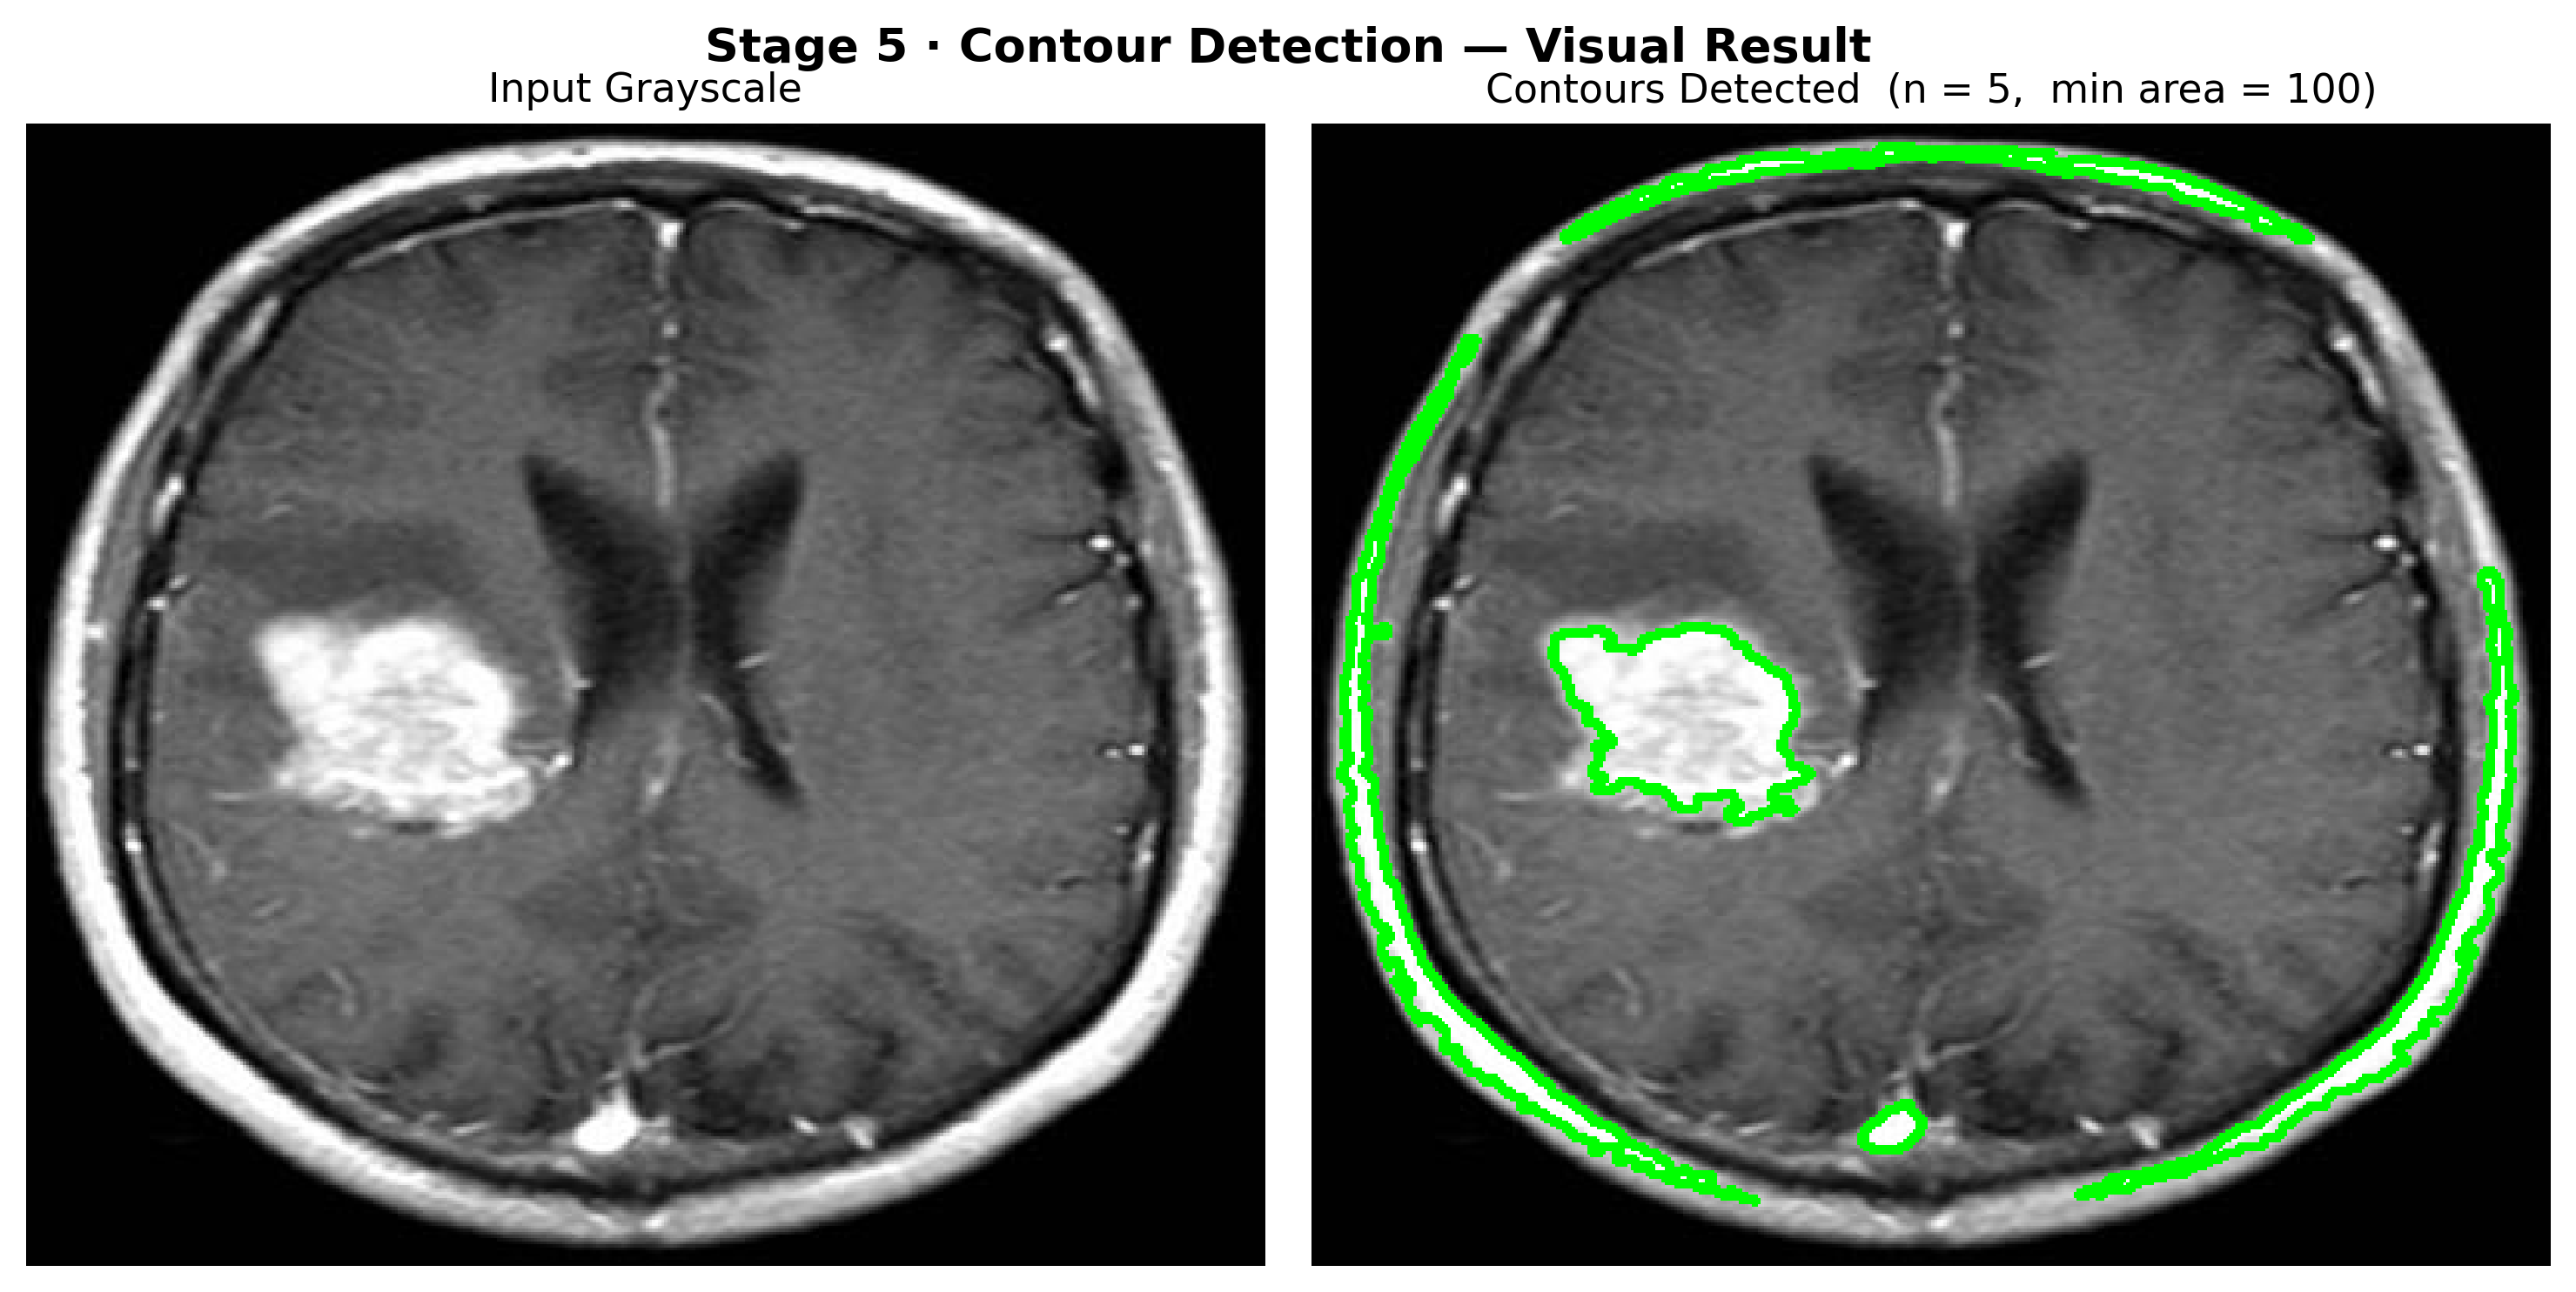
\includegraphics[width=0.96\textwidth,height=0.80\textheight,
                     keepaspectratio]{image-processor/contour_comparison.png}
\end{frame}

% ===== SECTION 4 =====
\section{Results}

\begin{frame}{Image Quality Metrics Analysis}
    \centering
    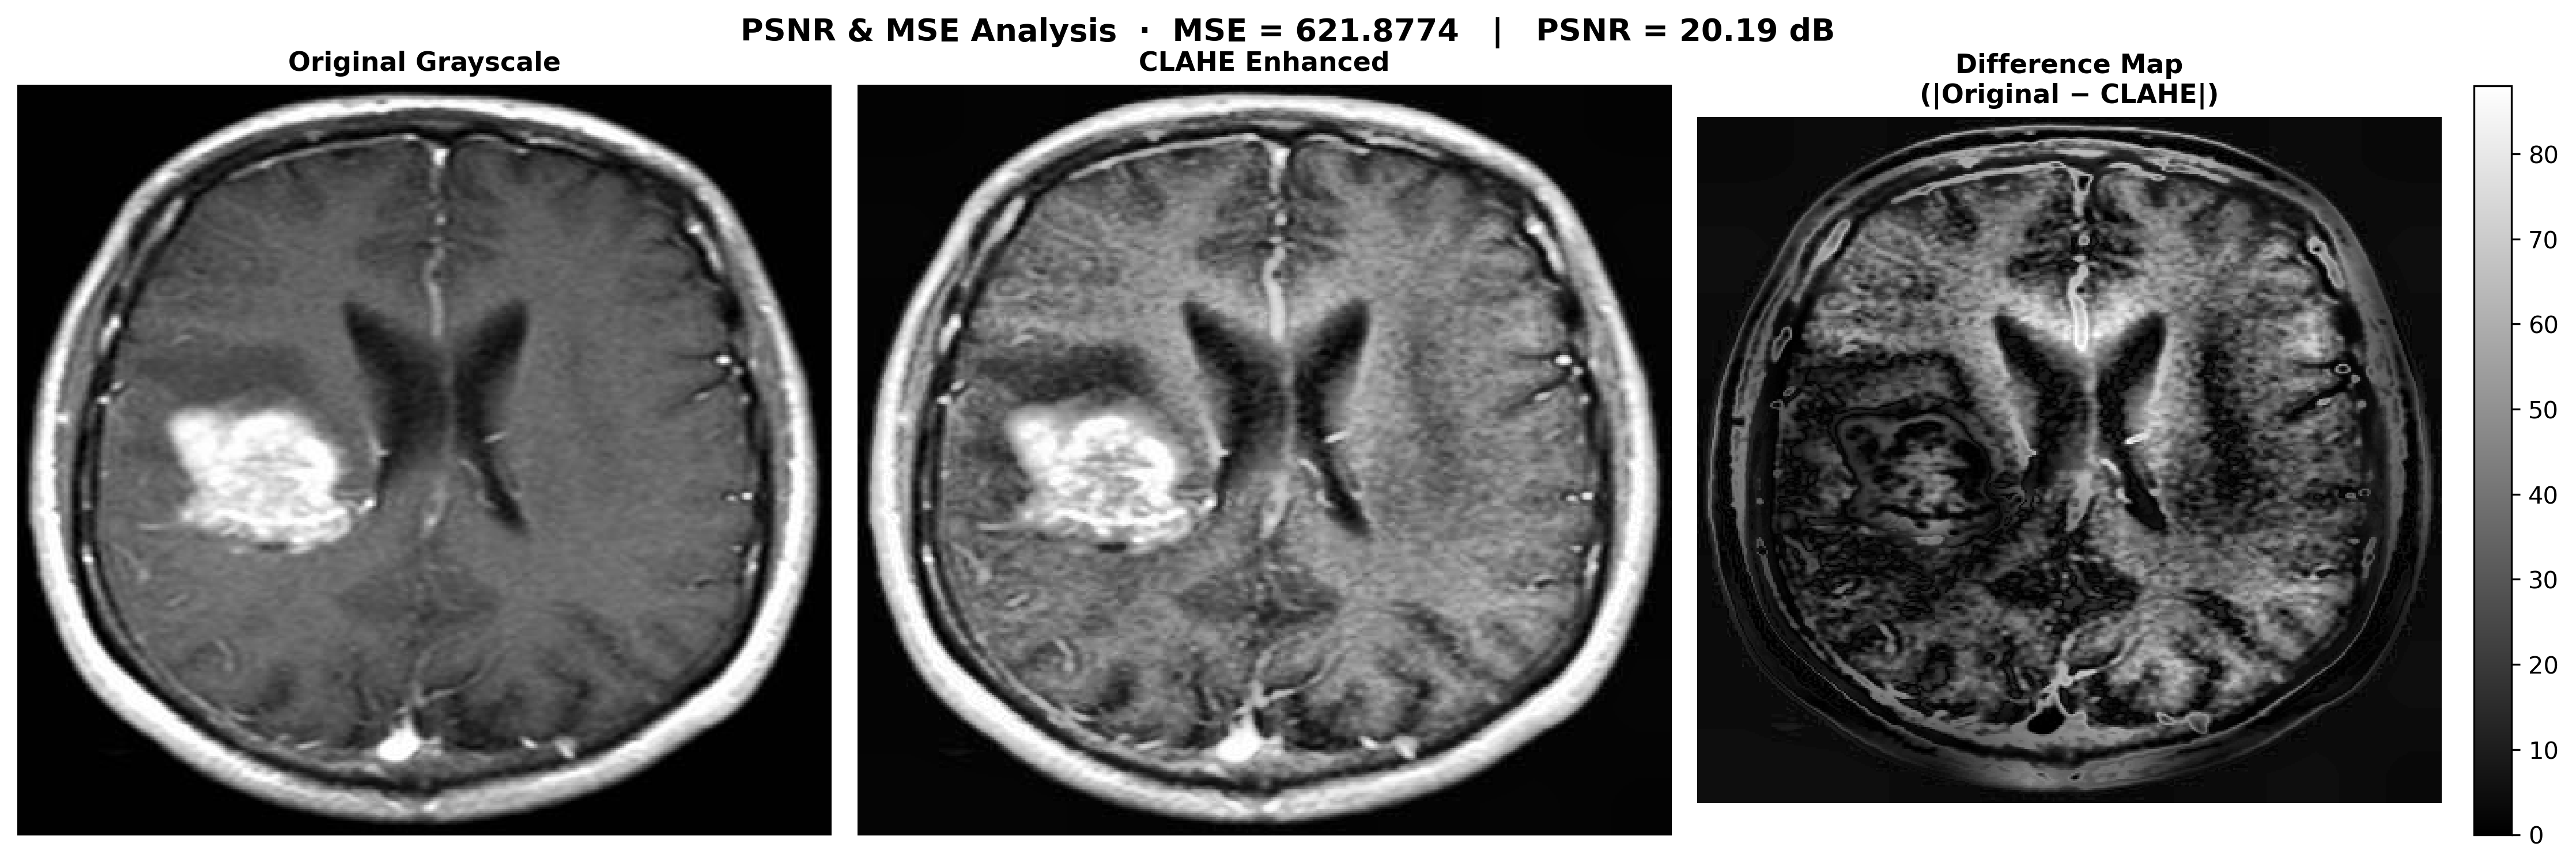
\includegraphics[width=0.96\textwidth,height=0.80\textheight,
                     keepaspectratio]{image-processor/psnr_mse_analysis.png}
\end{frame}

\begin{frame}{Quality Metrics -- Interpretation}
  \begin{columns}[T]
    \column{0.50\textwidth}
    \textbf{Measured Values:}
    \vspace{0.3cm}

    % ── KEY FIX: no \\[Xpt] inside node text; use \vspace instead ──
    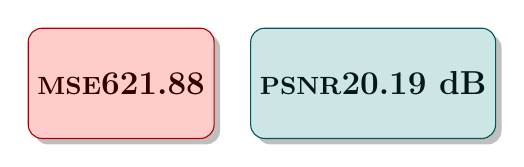
\begin{tikzpicture}
      \node[metricbox=red, minimum width=2.2cm] (mse) at (0,0) {%
        MSE\vspace{3pt}\par\large 621.88};
      \node[metricbox=teal, minimum width=2.2cm] (psnr) at (3.2,0) {%
        PSNR\vspace{3pt}\par\large 20.19 dB};
    \end{tikzpicture}

    \vspace{0.35cm}
    \begin{itemize}\setlength\itemsep{3pt}
        \item Avg.\ pixel difference $\approx$ 25 units (0--255)
        \item \textbf{Expected} for aggressive feature extraction
        \item Reflects intentional structural modification
    \end{itemize}

    \column{0.46\textwidth}
    \textbf{Clinical Context:}
    \begin{itemize}\setlength\itemsep{3pt}
        \item Goal is feature clarity, not signal fidelity
        \item Lower PSNR indicates successful extraction
        \item Trade-off: preservation vs.\ diagnostics
    \end{itemize}
    \vspace{0.3cm}
    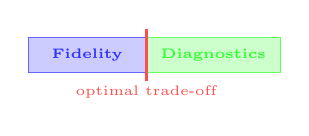
\begin{tikzpicture}
      \draw[fill=blue!20,draw=blue!60](0,0)rectangle(1.5,0.45)
            node[midway,font=\tiny\bfseries,text=blue!80]{Fidelity};
      \draw[fill=green!20,draw=green!60](1.5,0)rectangle(3.2,0.45)
            node[midway,font=\tiny\bfseries,text=green!80]{Diagnostics};
      \draw[very thick,red!70](1.5,-0.1)--(1.5,0.55);
      \node[font=\tiny,text=red!70]at(1.5,-0.25){optimal trade-off};
    \end{tikzpicture}
  \end{columns}
\end{frame}

\begin{frame}{PSNR / MSE Comparative Analysis}
    \centering
    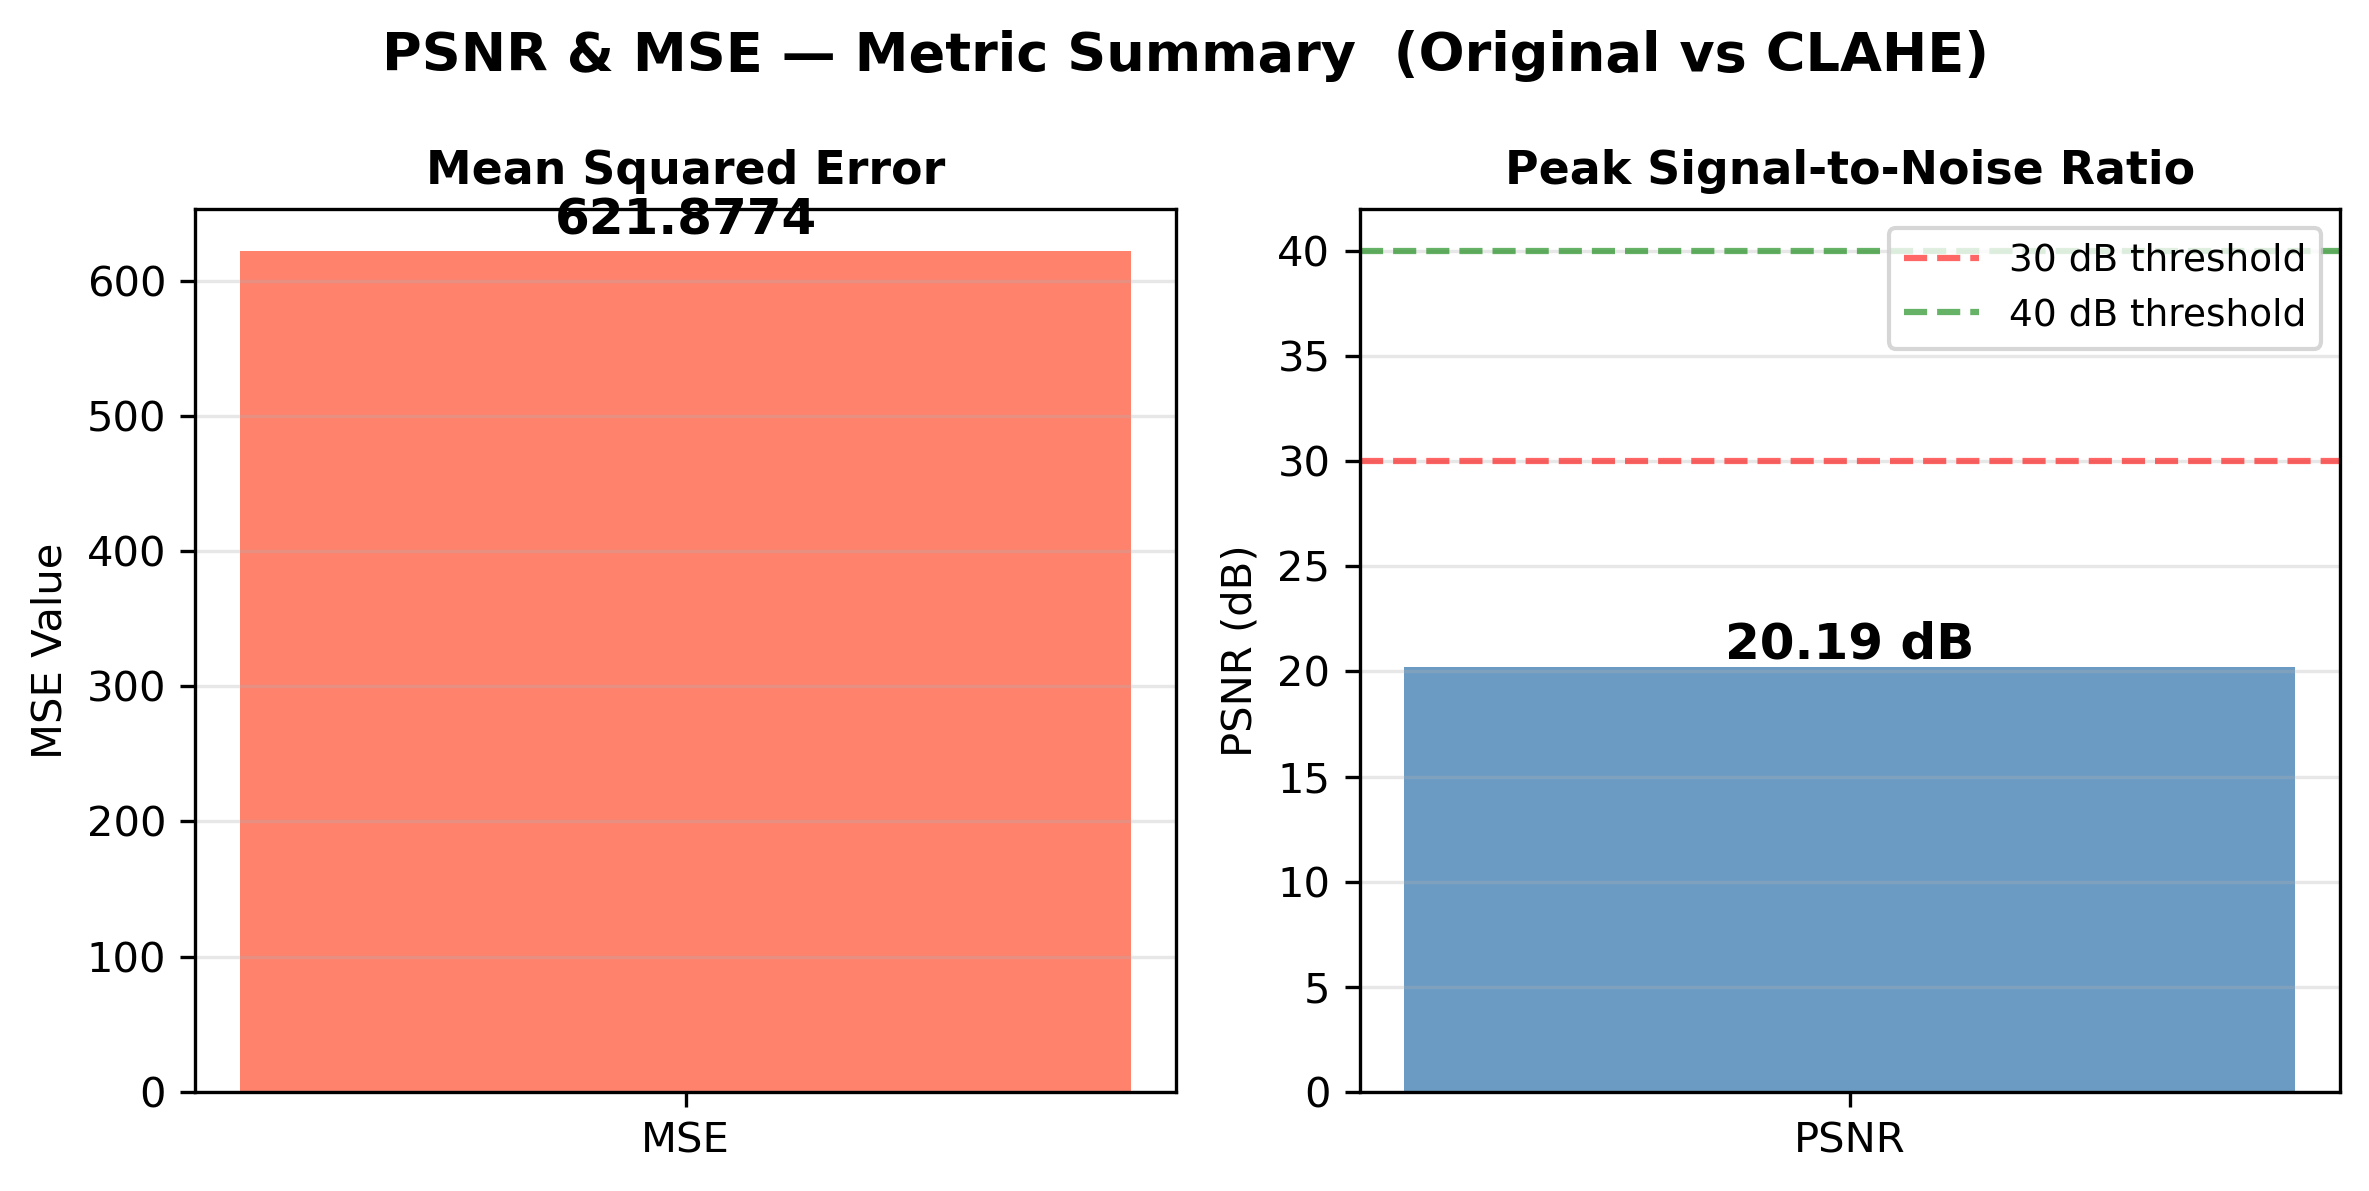
\includegraphics[width=0.96\textwidth,height=0.80\textheight,
                     keepaspectratio]{image-processor/psnr_mse_bars.png}
\end{frame}

% ===== SECTION 5 =====
\section{Mathematical Foundation}

\begin{frame}{Quality Assessment Equations}
    \textbf{Mean Squared Error (MSE):}
    \[
        \text{MSE} = \frac{1}{M \times N}
        \sum_{i=0}^{M-1}\sum_{j=0}^{N-1}
        \bigl[I_{\text{orig}}(i,j) - I_{\text{proc}}(i,j)\bigr]^{2}
    \]
    \vspace{0.3cm}
    \textbf{Peak Signal-to-Noise Ratio (PSNR):}
    \[
        \text{PSNR} = 10\log_{10}\!\left(\frac{\text{MAX}^{2}}{\text{MSE}}\right)
        \quad \text{where MAX} = 255
    \]
    \vspace{0.25cm}
    \centering
    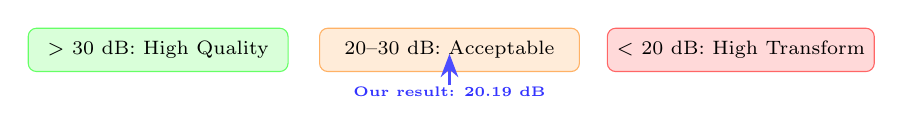
\begin{tikzpicture}
      \node[rectangle,rounded corners=3pt,draw=green!60,fill=green!15,
            minimum width=3.3cm,minimum height=0.55cm,font=\scriptsize]
            at(-3.7,0){$>$ 30 dB: High Quality};
      \node[rectangle,rounded corners=3pt,draw=orange!60,fill=orange!15,
            minimum width=3.3cm,minimum height=0.55cm,font=\scriptsize]
            at(0,0){20--30 dB: Acceptable};
      \node[rectangle,rounded corners=3pt,draw=red!60,fill=red!15,
            minimum width=3.3cm,minimum height=0.55cm,font=\scriptsize]
            at(3.7,0){$<$ 20 dB: High Transform};
      \draw[very thick,blue!70,-Stealth](0,-0.45)--(0,-0.05)
            node[below=8pt,font=\tiny\bfseries,text=blue!80]{Our result: 20.19 dB};
    \end{tikzpicture}
\end{frame}

% ===== SECTION 6 =====
\section{Sustainable Development Goals}

\begin{frame}{SDG Alignment}
  \centering
  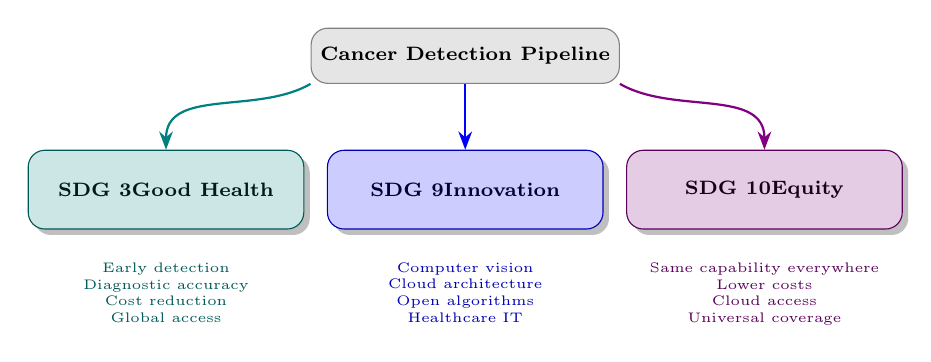
\begin{tikzpicture}[node distance=0.4cm and 0.5cm]
    \node[rectangle,rounded corners=6pt,fill=gray!20,draw=gray,
          minimum width=3.2cm,minimum height=0.7cm,
          font=\scriptsize\bfseries](proj)at(3.8,2.5){Cancer Detection Pipeline};
    \node[sdgbox=teal]  (s3)  at(0,0.8)  {SDG 3\\Good Health};
    \node[sdgbox=blue]  (s9)  at(3.8,0.8) {SDG 9\\Innovation};
    \node[sdgbox=violet](s10) at(7.6,0.8){SDG 10\\Equity};
    \draw[pipearrow,teal]  (proj.south west)to[out=210,in=90](s3.north);
    \draw[pipearrow,blue]  (proj.south)--(s9.north);
    \draw[pipearrow,violet](proj.south east)to[out=330,in=90](s10.north);
    \node[below=0.3cm of s3, font=\tiny,text=teal!70!black,
          align=center,text width=3.2cm]
         {Early detection\\Diagnostic accuracy\\Cost reduction\\Global access};
    \node[below=0.3cm of s9, font=\tiny,text=blue!70!black,
          align=center,text width=3.2cm]
         {Computer vision\\Cloud architecture\\Open algorithms\\Healthcare IT};
    \node[below=0.3cm of s10,font=\tiny,text=violet!70!black,
          align=center,text width=3.2cm]
         {Same capability everywhere\\Lower costs\\Cloud access\\Universal coverage};
  \end{tikzpicture}
\end{frame}

% ===== SECTION 7 =====
\section{Future Enhancements}

\begin{frame}{Future Roadmap}
  \centering
  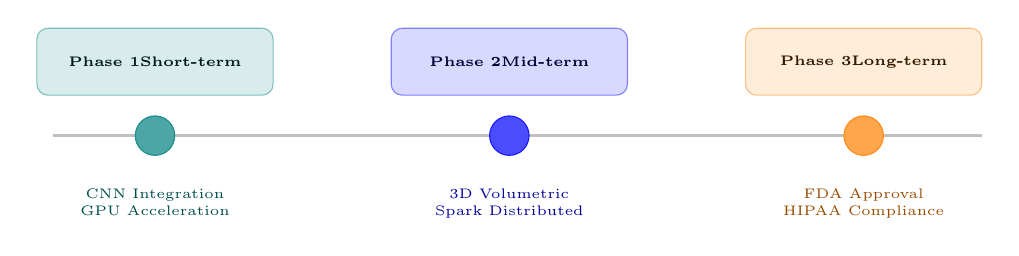
\begin{tikzpicture}
    \draw[very thick,gray!50](-0.3,0)--(11.5,0);
    % Phase 1
    \node[circle,fill=teal!70,draw=teal!90,minimum size=0.5cm,
          text=white,font=\tiny\bfseries](c1)at(1.0,0){};
    \node[rectangle,rounded corners=4pt,fill=teal!15,draw=teal!50,
          minimum width=3.0cm,minimum height=0.85cm,
          font=\tiny\bfseries,text=teal!20!black,above=0.25cm of c1]
         {Phase 1\\Short-term};
    \node[font=\tiny,text=teal!60!black,below=0.3cm of c1,
          text width=3.0cm,align=center]{CNN Integration\\GPU Acceleration};
    % Phase 2
    \node[circle,fill=blue!70,draw=blue!90,minimum size=0.5cm,
          text=white,font=\tiny\bfseries](c2)at(5.5,0){};
    \node[rectangle,rounded corners=4pt,fill=blue!15,draw=blue!50,
          minimum width=3.0cm,minimum height=0.85cm,
          font=\tiny\bfseries,text=blue!20!black,above=0.25cm of c2]
         {Phase 2\\Mid-term};
    \node[font=\tiny,text=blue!60!black,below=0.3cm of c2,
          text width=3.0cm,align=center]{3D Volumetric\\Spark Distributed};
    % Phase 3
    \node[circle,fill=orange!70,draw=orange!90,minimum size=0.5cm,
          text=white,font=\tiny\bfseries](c3)at(10.0,0){};
    \node[rectangle,rounded corners=4pt,fill=orange!15,draw=orange!50,
          minimum width=3.0cm,minimum height=0.85cm,
          font=\tiny\bfseries,text=orange!20!black,above=0.25cm of c3]
         {Phase 3\\Long-term};
    \node[font=\tiny,text=orange!60!black,below=0.3cm of c3,
          text width=3.0cm,align=center]{FDA Approval\\HIPAA Compliance};
  \end{tikzpicture}
  \vspace{0.5cm}
  \begin{columns}
    \column{0.32\textwidth}\centering
      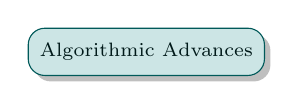
\begin{tikzpicture}
        \node[sdgbox=teal,minimum width=3.0cm,minimum height=0.6cm,
              font=\scriptsize]{Algorithmic Advances};
      \end{tikzpicture}
    \column{0.32\textwidth}\centering
      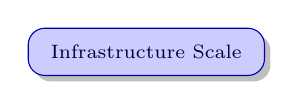
\begin{tikzpicture}
        \node[sdgbox=blue,minimum width=3.0cm,minimum height=0.6cm,
              font=\scriptsize]{Infrastructure Scale};
      \end{tikzpicture}
    \column{0.32\textwidth}\centering
      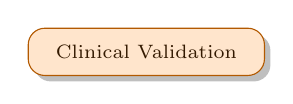
\begin{tikzpicture}
        \node[sdgbox=orange,minimum width=3.0cm,minimum height=0.6cm,
              font=\scriptsize]{Clinical Validation};
      \end{tikzpicture}
  \end{columns}
\end{frame}

% ===== SECTION 8 =====
\section{Conclusions}

\begin{frame}{Key Achievements}
    \begin{columns}[T]
        \column{0.48\textwidth}
        \textbf{Technical Success:}
        \begin{itemize}\setlength\itemsep{4pt}
            \item 6-stage pipeline fully implemented
            \item Multi-feature extraction working
            \item Quantitative metrics computed
            \item Cloud-native architecture deployed
        \end{itemize}
        \column{0.48\textwidth}
        \textbf{Clinical Impact:}
        \begin{itemize}\setlength\itemsep{4pt}
            \item Objective analysis capability
            \item Early detection support
            \item Accessible technology platform
            \item SDG 3, 9 and 10 alignment
        \end{itemize}
    \end{columns}
    \vspace{0.4cm}
    \centering
    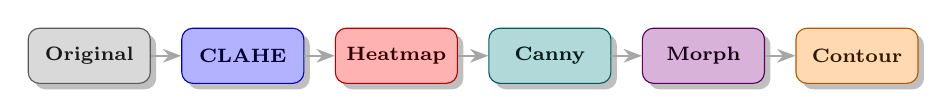
\begin{tikzpicture}
      \node[pipenode=gray,  minimum width=1.55cm,minimum height=0.7cm](r0)at(0,0)    {Original};
      \node[pipenode=blue,  minimum width=1.55cm,minimum height=0.7cm](r1)at(1.95,0) {CLAHE};
      \node[pipenode=red,   minimum width=1.55cm,minimum height=0.7cm](r2)at(3.90,0) {Heatmap};
      \node[pipenode=teal,  minimum width=1.55cm,minimum height=0.7cm](r3)at(5.85,0) {Canny};
      \node[pipenode=violet,minimum width=1.55cm,minimum height=0.7cm](r4)at(7.80,0) {Morph};
      \node[pipenode=orange,minimum width=1.55cm,minimum height=0.7cm](r5)at(9.75,0) {Contour};
      \draw[pipearrow](r0.east)--(r1.west);
      \draw[pipearrow](r1.east)--(r2.west);
      \draw[pipearrow](r2.east)--(r3.west);
      \draw[pipearrow](r3.east)--(r4.west);
      \draw[pipearrow](r4.east)--(r5.west);
    \end{tikzpicture}
\end{frame}

\begin{frame}{Project Vision}
    \centering
    \large\textbf{From Research to Global Impact}
    \vspace{0.5cm}

    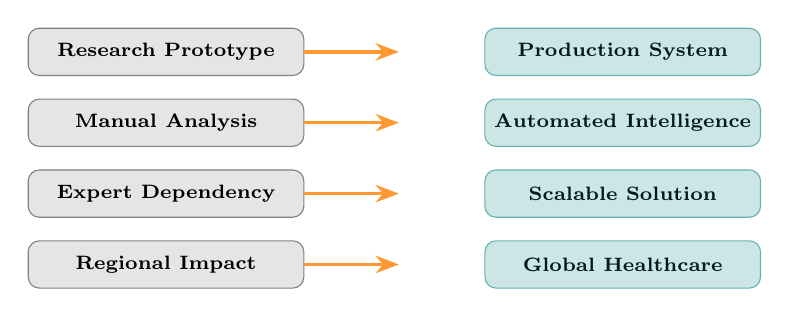
\begin{tikzpicture}
      \node[rectangle,rounded corners=4pt,fill=gray!20,draw=gray,
            minimum width=3.5cm,minimum height=0.6cm,font=\scriptsize\bfseries]
            (a1)at(0, 0)   {Research Prototype};
      \node[rectangle,rounded corners=4pt,fill=gray!20,draw=gray,
            minimum width=3.5cm,minimum height=0.6cm,font=\scriptsize\bfseries]
            (a2)at(0,-0.9) {Manual Analysis};
      \node[rectangle,rounded corners=4pt,fill=gray!20,draw=gray,
            minimum width=3.5cm,minimum height=0.6cm,font=\scriptsize\bfseries]
            (a3)at(0,-1.8) {Expert Dependency};
      \node[rectangle,rounded corners=4pt,fill=gray!20,draw=gray,
            minimum width=3.5cm,minimum height=0.6cm,font=\scriptsize\bfseries]
            (a4)at(0,-2.7) {Regional Impact};
      \draw[-Stealth,very thick,orange!80](a1.east)--++(1.2,0);
      \draw[-Stealth,very thick,orange!80](a2.east)--++(1.2,0);
      \draw[-Stealth,very thick,orange!80](a3.east)--++(1.2,0);
      \draw[-Stealth,very thick,orange!80](a4.east)--++(1.2,0);
      \node[rectangle,rounded corners=4pt,fill=teal!20,draw=teal!60,
            minimum width=3.5cm,minimum height=0.6cm,font=\scriptsize\bfseries,
            text=teal!20!black]at(5.8, 0)  {Production System};
      \node[rectangle,rounded corners=4pt,fill=teal!20,draw=teal!60,
            minimum width=3.5cm,minimum height=0.6cm,font=\scriptsize\bfseries,
            text=teal!20!black]at(5.8,-0.9){Automated Intelligence};
      \node[rectangle,rounded corners=4pt,fill=teal!20,draw=teal!60,
            minimum width=3.5cm,minimum height=0.6cm,font=\scriptsize\bfseries,
            text=teal!20!black]at(5.8,-1.8){Scalable Solution};
      \node[rectangle,rounded corners=4pt,fill=teal!20,draw=teal!60,
            minimum width=3.5cm,minimum height=0.6cm,font=\scriptsize\bfseries,
            text=teal!20!black]at(5.8,-2.7){Global Healthcare};
    \end{tikzpicture}
\end{frame}

% ===== QUESTIONS =====
\begin{frame}{Questions?}
    \vspace{0.4cm}
    \centering
    \LARGE\textbf{Questions and Discussion}
    \vspace{0.7cm}

    \normalsize
    \begin{tabular}{ll}
        \textbf{Repository:} &
        \texttt{github.com/Muhammad-Ahmad17/cancer\_cells} \\[8pt]
        \textbf{Contact:}    &
        \texttt{muhammadahmad171105@gmail.com}              \\
    \end{tabular}

    \vspace{0.7cm}
    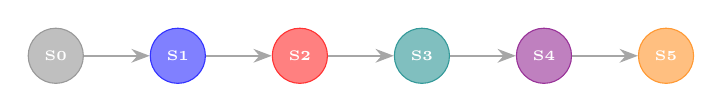
\begin{tikzpicture}
      \node[circle,fill=gray!50,  draw=gray!80,  minimum size=0.7cm,
            font=\tiny\bfseries,text=white](c0)at(0,0)   {S0};
      \node[circle,fill=blue!50,  draw=blue!80,  minimum size=0.7cm,
            font=\tiny\bfseries,text=white](c1)at(1.55,0){S1};
      \node[circle,fill=red!50,   draw=red!80,   minimum size=0.7cm,
            font=\tiny\bfseries,text=white](c2)at(3.10,0){S2};
      \node[circle,fill=teal!50,  draw=teal!80,  minimum size=0.7cm,
            font=\tiny\bfseries,text=white](c3)at(4.65,0){S3};
      \node[circle,fill=violet!50,draw=violet!80,minimum size=0.7cm,
            font=\tiny\bfseries,text=white](c4)at(6.20,0){S4};
      \node[circle,fill=orange!50,draw=orange!80,minimum size=0.7cm,
            font=\tiny\bfseries,text=white](c5)at(7.75,0){S5};
      \draw[pipearrow](c0.east)--(c1.west);
      \draw[pipearrow](c1.east)--(c2.west);
      \draw[pipearrow](c2.east)--(c3.west);
      \draw[pipearrow](c3.east)--(c4.west);
      \draw[pipearrow](c4.east)--(c5.west);
    \end{tikzpicture}
\end{frame}

\end{document}